\section{Modeling a Biological System }
\label{Modeling a Biological System }




This example was inspired by a paper that uses an adaptation of the UKF, called the Iterative Unscented Kalman Filter (IUKF), to model the biological pathway of metabolites, which are molecules that are the byproduct of the body's metabolism. This model contained four different states, or metabolites, which contained 18 unknown parameters. These researchers utilized the IUKF for parameter fitting and was useful in enabling the model converge faster by resetting the covariance to re-excite the model. Utilizing the IUKF on this model was effective, because data regarding metabolites is highly influenced by noise, which is a factor that makes other approaches, such as regression and annealing, fail \cite{article5} \\ 

\noindent By skipping this step (as is done in the UKF), the three state variables without measurements converge significantly slower. A metabolite is small bodily structure that is the byproduct of the metabolism. Data regarding metabolites is highly influenced by noise, which is a factor that makes other approaches, such as regression and annealing, fail \cite{article5}. \\ 

\noindent In the paper, researchers had access to their own data sources and used an approach that was adapted from the UKF. Though we are not using their exact dataset, we will be simulating data using the same approach as the previous example. However, this example will be following UKF algorithm, as opposed to the IUKF algorithm. By doing so, the state variables without incoming measurements converge significantly slower than the measurable states. Ultimately, the three goals of this example is to demonstrate how the UKF works on higher dimensional and more complex systems, how the UKF can correct for multiple variables or states, and how parameters can be adjusted to fit the model. \\ 

\noindent In this example, four metabolites, or states, are have the following differential equations:
\begin{align*}
\dot x_1 &= \alpha_1 x_3^{g_{13}} x_5^{g_{15}} - \beta_1 x_1^{h_{11}}, \\
\dot x_2 &= \alpha_2 x_1^{g_{21}} - \beta_2 x_2^{h_{22}}, \\
\dot x_3 &= \alpha_3 x_2^{g_{32}} - \beta_3 x_3^{h_{33}} x_4^{h_{34}}, \\
\dot x_4 &= \alpha_4  x_1^{g_{41}} - \beta_4 x_4^{h_{44}},
\end{align*}
where there are 18 unknown parameters ($\alpha_1, \hdots, \alpha_4, \beta_1, \hdots, \beta_4, g_{13}, g_{15}, g_{21}, \\ g_{32}, g_{41}, h_{11}, h_{22}, h_{33}, h_{34}, h_{44} $). We have a guess as to what these values might be and we will use the UKF to find parameter values that best fit model to some state. In both the original example as well as this one, sampling time will be 0.1 seconds for 5 seconds, totaling 50 UKF estimates. \\ \\

\noindent Since we did not have access to the original example's dataset, data was simulated on MATLAB. Similar to the previous example, the system's true output was simulated using an ODE solver and incoming system measurements were calculated by adding noise to the true value. The model was initialized by setting the state variable to $x_0 = [4, 1, 3, 4]^T$ and the state covariance to $P_0 = .01I$.

\newpage

\begin{center}
\begin{table}

\caption{True Parameter Values} \label{tab:sometab}
\begin{tabular}{ |P{1cm}||P{1cm} P{1cm} P{1cm} P{1cm} P{1cm} P{1cm} P{1cm} P{1cm} P{1cm} P{1cm}|}
    \hline
    \multicolumn{11}{|c|}{True Parameter Values} \\ 
    \hline
      & $\alpha_i$ & $g_{i1}$ & $g_{i2}$ & $g_{i3}$ & $g_{i4}$ & $\beta_i$ & $h_{i1}$ & $h_{i2}$ & $h_{i3}$ & $h_{i4}$\\
    \hline
    $x_1$ & 20.0  & 0 & 0 & -0.8 & 0 & 10.0 & 0.5 & 0 & 0 & 0\\
    $x_2$ & 8.0  & .5  & 0 & 0 & 0 & 3.0 & 0 & 0.75 & 0 & 0\\
    $x_3$ & 3.0  & 0 & 0.75 & 0 & 0 & 5.0 & 0 & 0 & 0.5 & 0.2\\
    $x_4$ & 2.0 & .5  & 0 & 0 & 0 & 6.0 & 0 & 0 & 0 & 0.8\\
    
    \hline
\end{tabular}

\end{table}
\end{center}


\begin{figure}[h]
    \centering
    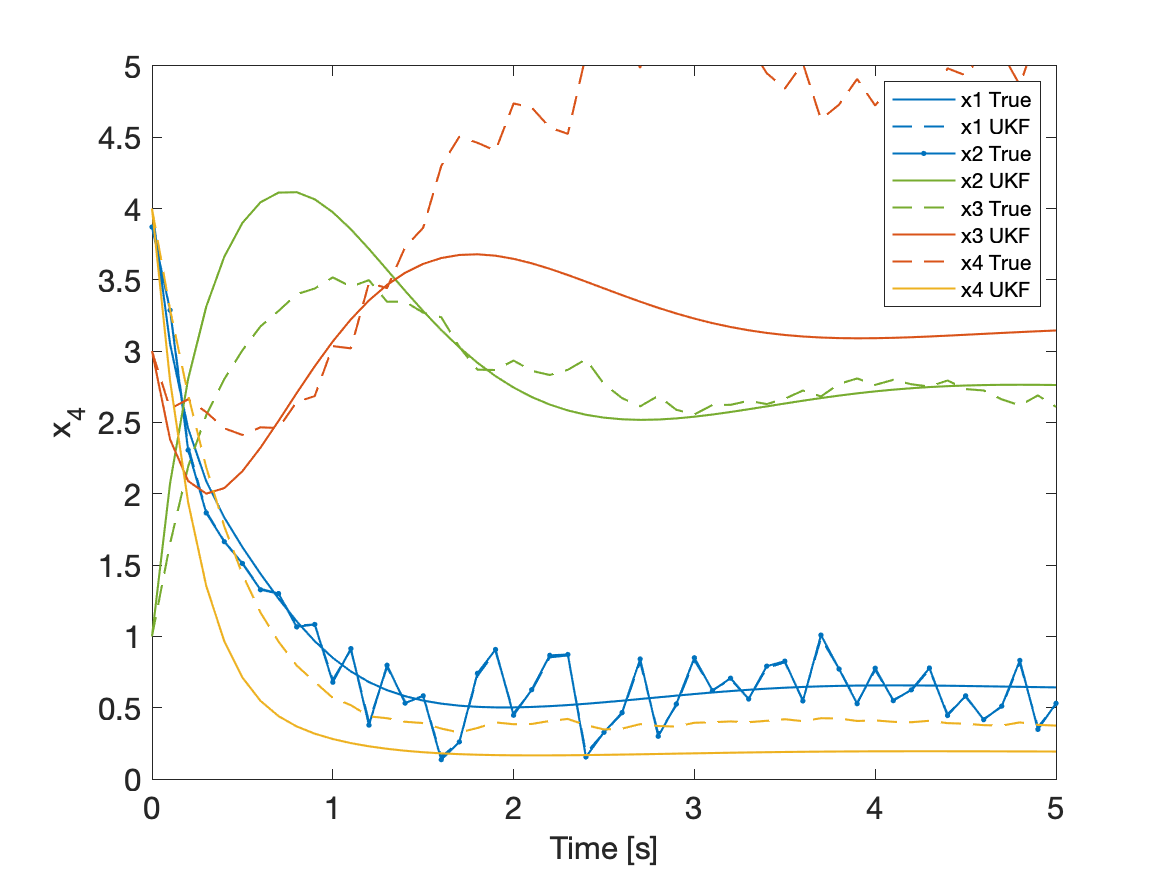
\includegraphics[scale = 0.6]{Meskin_overall.png}
    \caption{Performance of all state variables with the following conditions: R = 0.001, Q = (0.02 0.01 .03 .04) and initial values = $[4, 1, 3, 4]^T$.}
    %Paramaters included:  }% $, \alpha = 1, \kappa = 0  }
\end{figure}




\newpage

\begin{figure}[h]
    \centering
    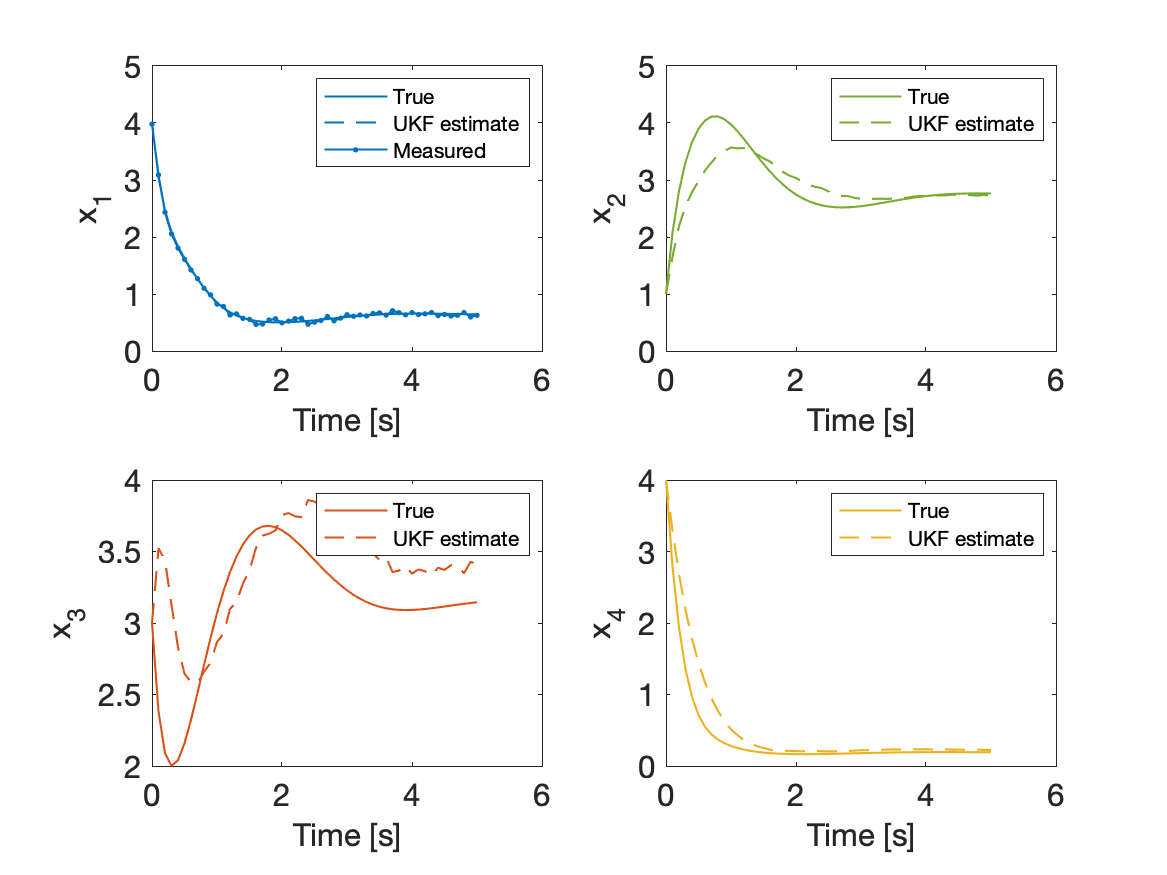
\includegraphics[scale = 0.6]{Meskin_states.png}
    \caption{Performance of all four state variables with one corrected state. The first state variable (blue) is the only one that is receiving measurements from the system. This explains why it is more accurate and converges better with the system, as compared with the other three states.}
    \label{map}
\end{figure}

\begin{figure}[h]
    \centering
    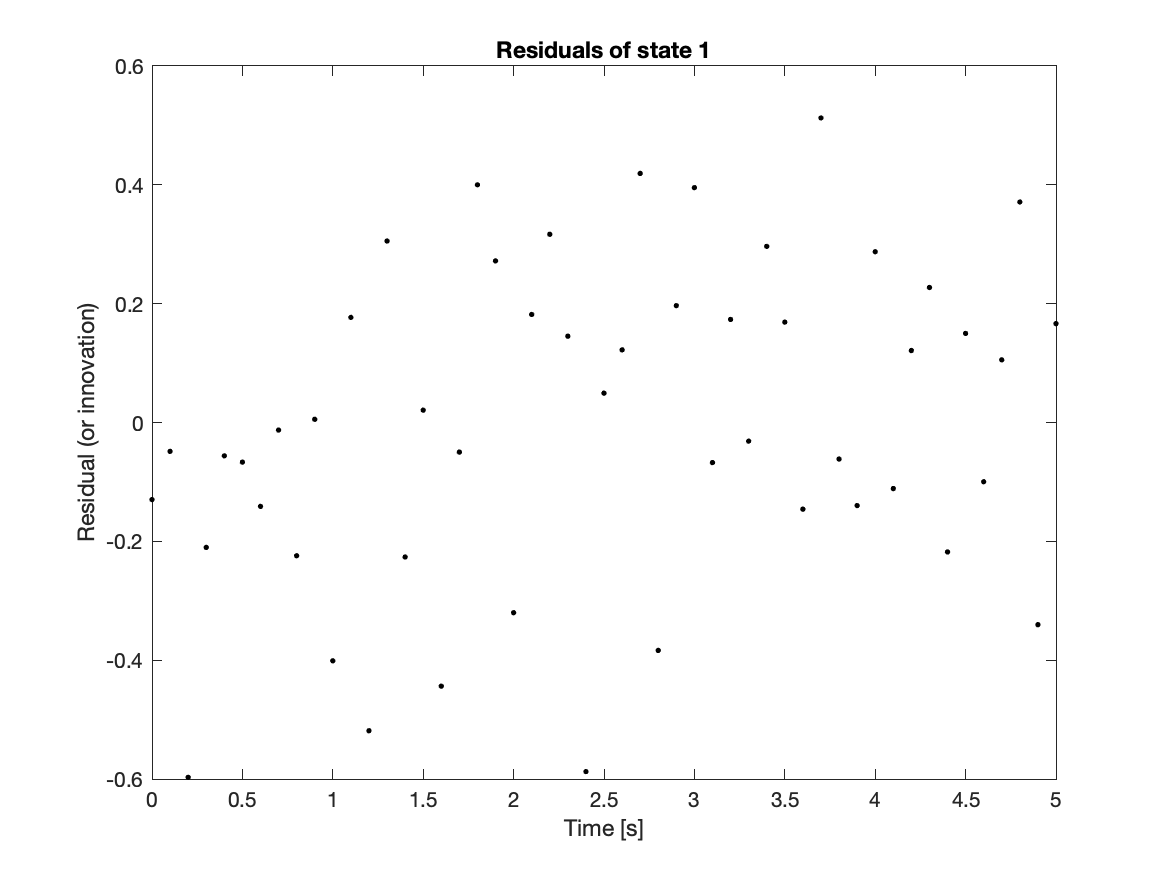
\includegraphics[scale = 0.6]{Meskin_residuals_state1.png}
    \caption{This scatterplot provides information regarding the residual, or innovation, of the first state, which is the only state recieving incoming system measurements.}
\end{figure}


\noindent \textcolor{red}{Expand here on tweaking parameters}.In the original example, researchers used the following parameter values: $\epsilon = 1, \kappa = -14$. In theory, values of $\kappa$ can be negative, but negative values cannot be inputted into MATLAB. Therefore, the parameter values used in this example are set to \noindent \textcolor{red}{ADD PARAM VALUES HERE}.\\


\noindent \textcolor{red}{Expand here on correcting for 1+ states, currently we are having technical challenges in completing this step}













